% DO NOT COMPILE THIS FILE DIRECTLY!
% This is included by the other .tex files.

\begin{frame}[t,plain]
\titlepage
\end{frame}

\begin{frame}
\frametitle{Objects - or How We Learned to Stop Worrying and Love the Templates}
\begin{itemize}
   \item Attributes are a simple but powerful tool to describe data
   \item Lacking the capability to create containers around attributes describing a common concept
   \item The goal was to develop something semi-standardised, with the option to {\bf dynamically build templates}
   \item We have considered a list of different solutions such as simple boolean operators, but found that the current implementation was superior.
   \item The result is a simple template that uses the basic attriubte types as building blocks along with some meta data
   \item The template does {\bf not have to be known} in order to use the constructed objects
   \item What we maintain now is a set of common objects, but similarly to our other JSON formats, users can extend it with their own ideas.
\end{itemize}
\end{frame}

\begin{frame}
\frametitle{MISP Object Templates}
\begin{itemize}
\item Using a similar JSON format as the taxonomies, galaxies, warninglists.
\item You can find the default set of object templates in the git repository\footnote{\url{https://www.github.com/MISP/misp-objects/}}.
\item Some of the object templates capture objects from other standards or mimic the output of tools
\item We tried to capture the most common use-cases coming from our own use-case as well as those of various partners that got involved
\item Improvements or pull requests for new object templates are of course always welcome
\end{itemize}
\end{frame}

\begin{frame}
\frametitle{Existing Object examples}
\begin{itemize}
\item AIL-leak - {\bf AIL object, an example for an object catering to the output of another tool}
\item Android permission - {\bf An object used to further contextualise another object}
\item Bank account
\item File {\bf Generic object to describe a file}
\item Passive DNS
\item Regex
\item Sandbox report
\item Vulnerability {\bf Enabling new use-cases such as pre-sharing of vulnerability information}
\item x509
\item Yara {\bf Verbatim sharing of rule sets along with meta-data}
\end{itemize}
\end{frame}

\colorlet{punct}{red!60!black}
\definecolor{background}{HTML}{EEEEEE}
\definecolor{delim}{RGB}{20,105,176}
\colorlet{numb}{magenta!60!black}
\lstdefinelanguage{json}{
    basicstyle=\scriptsize,
    numbers=left,
    numberstyle=\scriptsize,
    stepnumber=1,
    numbersep=5pt,
    showstringspaces=false,
    breaklines=true,
    frame=lines,
    backgroundcolor=\color{background},
    literate=
     *{0}{{{\color{numb}0}}}{1}
      {1}{{{\color{numb}1}}}{1}
      {2}{{{\color{numb}2}}}{1}
      {3}{{{\color{numb}3}}}{1}
      {4}{{{\color{numb}4}}}{1}
      {5}{{{\color{numb}5}}}{1}
      {6}{{{\color{numb}6}}}{1}
      {7}{{{\color{numb}7}}}{1}
      {8}{{{\color{numb}8}}}{1}
      {9}{{{\color{numb}9}}}{1}
      {:}{{{\color{punct}{:}}}}{1}
      {,}{{{\color{punct}{,}}}}{1}
      {\{}{{{\color{delim}{\{}}}}{1}
      {\}}{{{\color{delim}{\}}}}}{1}
      {[}{{{\color{delim}{[}}}}{1}
      {]}{{{\color{delim}{]}}}}{1},
}

\begin{frame}[fragile]
\frametitle{Object Template skeleton}
\begin{lstlisting}[language=json,firstnumber=1]
{
  "requiredOneOf": [],
  "required": [],
  "attributes": {},
  "version": 1,
  "description": "My description",
  "meta-category": "Chosen meta category",
  "uuid": "Object template uuid",
  "name": "Object template name"
}
\end{lstlisting}
\end{frame}

\begin{frame}[fragile]
\frametitle{Adding elements to an object template}
\begin{lstlisting}[language=json,firstnumber=1]
"regexp-type": {
  "description": "Type of the regular expression syntax.",
  "disable_correlation": true,
  "ui-priority": 0,
  "misp-attribute": "text",
  "values_list": [
    "PCRE",
    "PCRE2",
    "POSIX BRE",
    "POSIX ERE"
  ]
},
\end{lstlisting}
\end{frame}

\begin{frame}
\frametitle{Attribute keys}
\begin{itemize}
\item Primary key: Object relation
\item description: A description of the attribute in relation to the object
\item disable\_correlation: You can disable correlations for attributes in the resulting object
\item ui-priority: Not implemented yet, but the idea is to have a "quick view" of objects only showing certain prio levels
\item misp-attribute: The misp attribute type used as as the building block
\item values\_list: an optional list of values from which the user {\bf must} choose instead of entering a value manually
\item sane\_defaults: an optional list of values from which the user {\bf may} choose instead of entering a value
\item multiple: Allow the user to add {\bf more} than one of this attribute
\end{itemize}
\end{frame}

\begin{frame}
\frametitle{Enforcement of certain keys}
\begin{itemize}
\item The template also defines which of the added attributes are mandatory
\item Requirements are pointed to via their {\bf object relations names}
\item We differentiate between two types of rule sets:
\begin{itemize}
\item Required: Everything in this list has to be set in order for the object to validate
\item Required One Of: Any of the attributes in this list will satisfy the requirements
\end{itemize}
\end{itemize}
\end{frame}

\begin{frame}
\frametitle{What will the template actually do?}
\begin{itemize}
\item Templates create a form that can be used to populate an event
\item When using templates, MISP will enforce everything according to the template rules
\item However, these are only optional, users can avoid using the templates when creating events via the API
\item The reason for this is that you do not need to have the template in order to create an object
\item The limitation of this system: You {\bf cannot modify} objects that were created with unknown templates
\end{itemize}
\end{frame}

\begin{frame}
\frametitle{Templates as rendered in the UI}
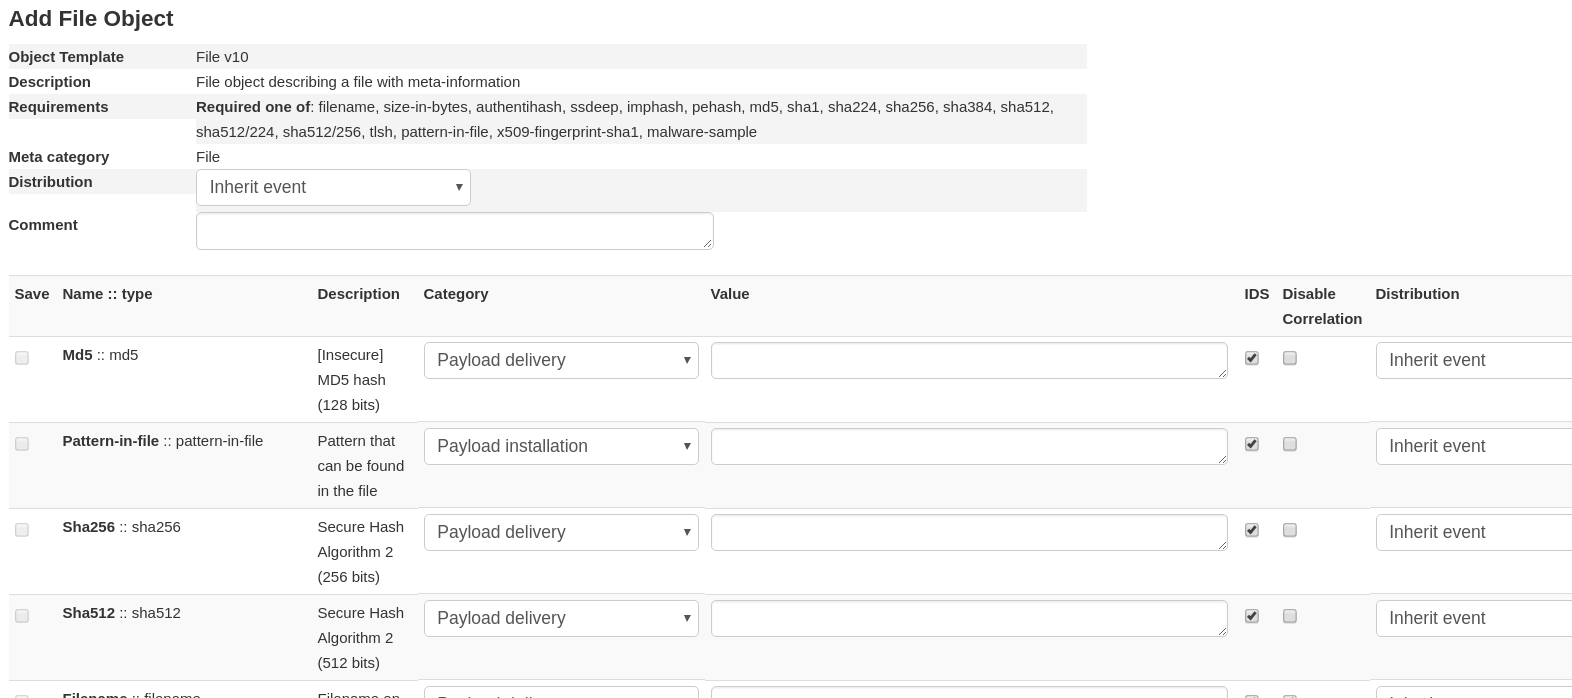
\includegraphics[scale=0.4]{template.png}
\end{frame}

\begin{frame}
\frametitle{Templates as rendered in the UI}
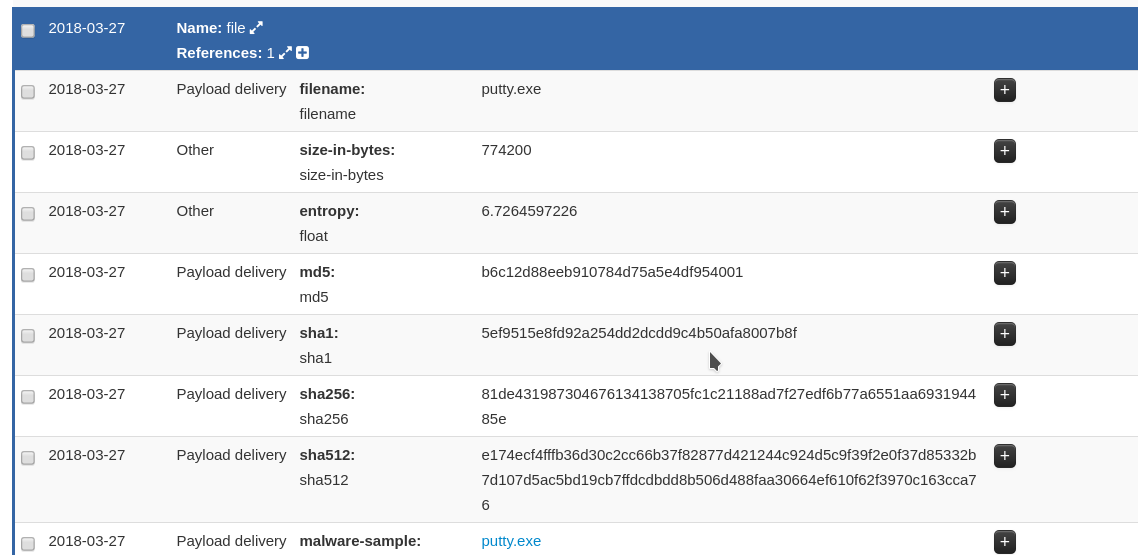
\includegraphics[scale=0.21]{object.png}
\end{frame}

\begin{frame}[t,fragile] {Q\&A}

\includegraphics[scale=0.5]{misplogo.pdf}
\begin{itemize}
        \item \url{https://github.com/MISP/MISP}
        \item \url{https://github.com/MISP/misp-objects}
        \item info@circl.lu (if you want to join one of the MISP community operated by CIRCL)
        \item PGP key fingerprint: CA57 2205 C002 4E06 BA70 BE89 EAAD CFFC 22BD 4CD5
\end{itemize}

\end{frame}

